\documentclass[aspectratio=169]{beamer}
\usepackage{tikz}
\usepackage{graphicx}
\usepackage{xypic}

\usecolortheme{whale}
\usetikzlibrary{er,positioning}  
\usetikzlibrary{decorations.pathreplacing}
\usetikzlibrary{arrows, decorations.markings}
\usetikzlibrary{shapes.geometric}
\usetikzlibrary{mindmap}

\setbeamertemplate{navigation symbols}{}

% \setbeameroption{show notes on second screen=right}

\definecolor{violet}{rgb}{0.53, 0.0, 0.69}

\definecolor{blue1}{RGB}{126,126,206}
\definecolor{blue2}{RGB}{87,87,192}
\definecolor{blue3}{RGB}{51,51,178}
\definecolor{blue4}{RGB}{27,26,107}

\tikzstyle{every link} = []
\tikzstyle{link} = [>=triangle 60, draw, every link]

\definecolor{attr}{RGB}{10,153,2}

\graphicspath{{img/}{./}} % Specifies where to look for included images (trailing slash required)

\title{Bases de Datos}
\subtitle{Dise\~no Correcto. Introducci\'on a SQL}
\author[Garc\'ia L., Cardentey V. M., Ledesma. A]{
    Lic. Andy Ledesma Garc\'ia\\ 
    Lic. V\'ictor M. Cardentey Fundora\\ 
    Dra. C. Lucina Garc\'ia Hern\'andez
}
\institute[MATCOM-UH]{
    Departamento de Computaci\'on\\
    Facultad de Matem\'atica y Computaci\'on\\
    Universidad de La Habana\\[3mm]
    Licenciatura en Ciencia de Datos
}
\date[]{20 de febrero de 2024}


\begin{document}
    \maketitle
    \begin{frame}{Continuemos con el ejemplo}
        $U = \{ \textnormal{\#E, ENombre,  Grupo, Provincia, \#A, ANombre, Nota}\}$

        $F = \{\textnormal{\#E} \to \textnormal{ENombre, Grupo, Provincia}${\bf;}\; $\textnormal{\#A} \to \textnormal{ANombre}${\bf;}\; $\textnormal{\#E,\#A} \to \textnormal{\#E,\#A}${\bf;}\; $\textnormal{\#E, \#A} \to \textnormal{Nota}${\bf;}\; $\textnormal{Provincia} \to \textnormal{Grupo}\}$\\[4mm]

    \centering
    \begin{tabular}{ccccccc}
        \underline{\#E} & ENombre & Grupo & Provincia & \underline{\#A} & ANombre & Nota\\
        $e_1$ & Juan & {111} & { La Habana} & $a_1$ & An\'alisis & 3\\
        $e_1$ & Juan & {111} & { La Habana} & $a_2$ & L\'ogica & 2\\
        $e_1$ & Juan & {111} & { La Habana} & $a_3$ & \'Algebra & 4\\
        $e_1$ & Juan & {111} & { La Habana} & $a_4$ & Programaci\'on & 5\\
        $e_3$ & Pedro & {111} & { La Habana} & $a_3$ & \'Algebra & 4\\
        $e_2$ & Mar\'ia & {112} & { Matanzas} & $a_1$ & An\'alisis & 3\\
        $e_2$ & Mar\'ia &  {112} & { Matanzas} & $a_2$ & L\'ogica & 3\\
        $e_4$ & Rita &  {112} & { Mayabeque} & $a_2$ & L\'ogica & 3\\
        $e_4$ & Rita &  {112} & { Mayabeque} & $a_4$ & Programaci\'on & 4\\
        $e_5$ & Carlos &  {113} & { Pinar del R\'io} & $a_3$ & \'Algebra & 3
    \end{tabular}

    \note{@NOTE alguien no depende completamente de la llave? Dependencias transitivas?}
\end{frame}

\begin{frame}{Recapitulando...}
    \vspace{-3mm}
    \begin{columns}[T]
        \begin{column}{0.68\linewidth}
            \begin{columns}[T]
                \begin{column}{0.6\textwidth}
                    \begin{center}
                        \textbf{Estudiante}\\[2mm]
        
                        \begin{tabular}{ccc}
                            \underline{\#E} & ENombre & Provincia\\[1mm]
                            \hline
                            $e_1$ & Juan & La Habana\\
                            $e_2$ & Mar\'ia & Matanzas\\
                            $e_3$ & Pedro & La Habana\\
                            $e_4$ & Rita & Mayabeque\\
                            $e_5$ & Carlos & Pinar del R\'io
                        \end{tabular}
                    \end{center}
                \end{column}

                \begin{column}{0.4\textwidth}
                    \begin{center}
                        \textbf{Provincia-Grupo}\\[2mm]
        
                        \begin{tabular}{cc}
                            \underline{Provincia} & Grupo\\[1mm]
                            \hline
                            La Habana & 111\\
                            Matanzas & 112 \\
                            Mayabeque & 112 \\
                            Pinar del R\'io & 113
                            
                        \end{tabular}
                    \end{center}
                \end{column}
                
            \end{columns}

            \begin{center}
                \textbf{Asignatura}\\[2mm]

                \begin{tabular}{cc}
                    \underline{\#A} & ANombre\\[1mm]
                    \hline
                    $a_1$ & An\'alisis\\
                    $a_2$ & L\'ogica \\
                    $a_3$ & \'Algebra\\
                    $a_4$ & Programaci\'on
                    
                \end{tabular}
            \end{center}
            
        \end{column}

        \begin{column}{0.3\linewidth}
            \vspace{6mm}
            \begin{center}
                \textbf{Evaluar}\\[2mm]

                \begin{tabular}{ccc}
                    \underline{\#E} & \underline{\#A} & Nota\\[1mm]
                    \hline
                    $e_1$ & $a_1$ & 3\\
                    $e_1$ & $a_2$ & 2\\
                    $e_1$ & $a_3$ & 4\\
                    $e_1$ & $a_4$ & 5\\
                    $e_3$ & $a_3$ & 4\\
                    $e_2$ & $a_1$ & 3\\
                    $e_2$ & $a_2$ & 3\\
                    $e_4$ & $a_2$ & 3\\
                    $e_4$ & $a_4$ & 4\\
                    $e_5$ & $a_3$ & 3\\
                \end{tabular}
            \end{center}
        \end{column}
    \end{columns}
    
    \note{@NOTE c\'omo obtenerla?}
\end{frame}


\begin{frame}{Que tan normalizado está el diseño?}
    \begin{block}{Primera Forma Normal}
        Un esquema relacional $R(U,F)$ est\'a en primera forma
        normal (1FN) si todos los atributos toman un solo valor del dominio
        subyacente.
        
    \end{block}
\end{frame}


\begin{frame}{Dependencia funcional completa}
    Dado un esquema relacional $R(U,F)$ y los atributos $X$, $Y$ de $R$
    (posiblemente compuestos), se dice que $Y$ depende funcional
    y completamente de $X$ si y solo si $Y$ depende funcionalmente de
    $X$ y no depende de alg\'un subconjunto propio de $X$.
\end{frame}

\begin{frame}{Clasificando dependencias}
    \centering
    \begin{columns}[T]
        \begin{column}{0.2\linewidth}
            
        \end{column}
        \begin{column}{0.3\linewidth}
            {\color<2>{blue}
            \#E, \#A $\to$ ENombre\\
            \#E, \#A $\to$ Grupo\\
            \#E, \#A $\to$ Provincia\\
            \#E, \#A $\to$ ANombre\\
            \vspace{1mm}
            }
            {\color<2>{orange}
            \#E, \#A $\to$ Nota\\
            \#E $\to$ ENombre\\
            \#E $\to$ Grupo\\
            \#E $\to$ Provincia\\
            \#A $\to$ ANombre\\
            Provincia $\to$ Grupo
            }
        \end{column}
        \begin{column}{0.3\linewidth}
            \onslide<2>{
            \vspace{5mm}
            \textcolor{blue}{\Large Incompletas}

            \vspace{20mm}
            \textcolor{orange}{\Large Completas}
            }
        \end{column}
        \begin{column}{0.2\linewidth}
            
        \end{column}
    \end{columns}
        
\end{frame}

\begin{frame}{Formas normales}
    \begin{block}{Segunda Forma Normal}
        Un esquema relacional $R(U,F)$ est\'a en segunda
        forma normal (2FN), si est\'a en 1FN y todos los atributos
        no llaves dependen completamente de la llave.
        
    \end{block}
\end{frame}

\begin{frame}{Llegando hasta segunda}
    \vspace{-5mm}
    \begin{columns}[T]
        \begin{column}{0.68\linewidth}
            \begin{center}
                \textbf{Estudiante}\\[2mm]

                \begin{tabular}{cccc}
                    \underline{\#E} & ENombre & Provincia & Grupo\\[1mm]
                    \hline
                    $e_1$ & Juan & La Habana & {\color<2>{red}111}\\
                    $e_2$ & Mar\'ia & Matanzas & 112\\
                    $e_3$ & Pedro & La Habana & {\color<2>{red}111}\\
                    $e_4$ & Rita & Mayabeque & 112\\
                    $e_5$ & Carlos & Pinar del R\'io & 113\\
                \end{tabular}
            \end{center}
            

               

            \begin{center}
                \textbf{Asignatura}\\[2mm]

                \begin{tabular}{cc}
                    \underline{\#A} & ANombre\\[1mm]
                    \hline
                    $a_1$ & An\'alisis\\
                    $a_2$ & L\'ogica \\
                    $a_3$ & \'Algebra\\
                    $a_4$ & Programaci\'on
                    
                \end{tabular}
            \end{center}
            
        \end{column}

        \begin{column}{0.3\linewidth}
            \vspace{6mm}
            \begin{center}
                \textbf{Evaluar}\\[2mm]

                \begin{tabular}{ccc}
                    \underline{\#E} & \underline{\#A} & Nota\\[1mm]
                    \hline
                    $e_1$ & $a_1$ & 3\\
                    $e_1$ & $a_2$ & 2\\
                    $e_1$ & $a_3$ & 4\\
                    $e_1$ & $a_4$ & 5\\
                    $e_3$ & $a_3$ & 4\\
                    $e_2$ & $a_1$ & 3\\
                    $e_2$ & $a_2$ & 3\\
                    $e_4$ & $a_2$ & 3\\
                    $e_4$ & $a_4$ & 4\\
                    $e_5$ & $a_3$ & 3\\
                \end{tabular}
            \end{center}
        \end{column}
    \end{columns}
\end{frame}

\begin{frame}{Llegando hasta segunda}
    \centering
    \Large \textcolor{red}{Todav\'ia existe redundancia innecesaria}
\end{frame}

\begin{frame}{Dependencia funcional transitiva}
    Dado un esquema relacional $R(U,F)$ y los atributos $X$, $Y$ y $Z$ de
    $R$ (posiblemente compuestos), se dice que $Z$ depende funcional
    y transitivamente de $X$ si y solo si $Y$ y $Z$ dependen funcionalmente
    de $X$ y, adem\'as, $Z$ depende funcionalmente de $Y$.

    Si $Z$ no dependiera funcionalmente de $Y$, entonces se dice que $Y$ y $Z$
    son mutuamente independientes.

    
\end{frame}

\begin{frame}{Dependencia funcional transitiva}

    \begin{columns}[T]
        \begin{column}{0.5\linewidth}
            \begin{center}
                \textbf{Estudiante}\\[2mm]

                \begin{tabular}{cccc}
                    \underline{\#E} & ENombre & Provincia & Grupo\\[1mm]
                    \hline
                    $e_1$ & Juan & La Habana & 111\\
                    $e_2$ & Mar\'ia & Matanzas & 112\\
                    $e_3$ & Pedro & La Habana & 111\\
                    $e_4$ & Rita & Mayabeque & 112\\
                    $e_5$ & Carlos & Pinar del R\'io & 113\\
                \end{tabular}
            \end{center}
            
        \end{column}

        \begin{column}{0.5\linewidth}
            \vspace{15mm}
            \hspace{5mm} \#E $\to$ ENombre\\
            \hspace{5mm} \#E $\to$ Grupo\\
            \hspace{5mm} \#E $\to$ Provincia\\
            \hspace{5mm} Provincia $\to$ Grupo
        \end{column}
        
        
    \end{columns}
    \vspace{5mm}

    \centering
    \onslide<2->{

        \#E $\to$ Provincia,  Provincia $\to$ Grupo $\models$ \#E $\to$ Grupo\\[2mm]
    }
    \onslide<3->{

        \Large \textcolor{red}{Existe una dependencia funcional transitiva}
    }
\end{frame}

\begin{frame}{Formas normales}
    \begin{block}{Tercera Forma Normal}
        Un esquema relacional $R(U,F)$ est\'a en tercera forma normal
        (3FN), si est\'a en 2FN y los atributos no llaves son mutuamente independientes.
        
    \end{block}
\end{frame}


\begin{frame}{Al fin, la tercera}
    \vspace{-3mm}
    \begin{columns}[T]
        \begin{column}{0.68\linewidth}
            \begin{columns}[T]
                \begin{column}{0.6\textwidth}
                    \begin{center}
                        \textbf{Estudiante}\\[2mm]
        
                        \begin{tabular}{ccc}
                            \underline{\#E} & ENombre & Provincia\\[1mm]
                            \hline
                            $e_1$ & Juan & La Habana\\
                            $e_2$ & Mar\'ia & Matanzas\\
                            $e_3$ & Pedro & La Habana\\
                            $e_4$ & Rita & Mayabeque\\
                            $e_5$ & Carlos & Pinar del R\'io
                        \end{tabular}
                    \end{center}
                \end{column}

                \begin{column}{0.4\textwidth}
                    \begin{center}
                        \textbf{Pronvincia-Grupo}\\[2mm]
        
                        \begin{tabular}{cc}
                            \underline{Provincia} & Grupo\\[1mm]
                            \hline
                            La Habana & 111\\
                            Matanzas & 112 \\
                            Mayabeque & 112 \\
                            Pinar del R\'io & 113
                            
                        \end{tabular}
                    \end{center}
                \end{column}
                
            \end{columns}

            \begin{center}
                \textbf{Asignatura}\\[2mm]

                \begin{tabular}{cc}
                    \underline{\#A} & ANombre\\[1mm]
                    \hline
                    $a_1$ & An\'alisis\\
                    $a_2$ & L\'ogica \\
                    $a_3$ & \'Algebra\\
                    $a_4$ & Programaci\'on
                    
                \end{tabular}
            \end{center}
            
        \end{column}

        \begin{column}{0.3\linewidth}
            \vspace{6mm}
            \begin{center}
                \textbf{Evaluar}\\[2mm]

                \begin{tabular}{ccc}
                    \underline{\#E} & \underline{\#A} & Nota\\[1mm]
                    \hline
                    $e_1$ & $a_1$ & 3\\
                    $e_1$ & $a_2$ & 2\\
                    $e_1$ & $a_3$ & 4\\
                    $e_1$ & $a_4$ & 5\\
                    $e_3$ & $a_3$ & 4\\
                    $e_2$ & $a_1$ & 3\\
                    $e_2$ & $a_2$ & 3\\
                    $e_4$ & $a_2$ & 3\\
                    $e_4$ & $a_4$ & 4\\
                    $e_5$ & $a_3$ & 3\\
                \end{tabular}
            \end{center}
        \end{column}
    \end{columns}
\end{frame}



\begin{frame}{Eliminando dependencias problem\'aticas}
    \begin{block}{Cubrimiento minimal}
        Dado dos conjuntos de dependencias funcionales $F$ y $G$, se dice
        que $G$ es un cubrimiento minimal o cobertura irreducible
        de $F$ si se cumple que:
        \begin{enumerate}
            \item $G \equiv F$
            \item $G$ no contiene atributos redundantes
            \item $G$ no contiene dependencias redundantes
        \end{enumerate}
        
    \end{block}
\end{frame}


{
\setbeamertemplate{background} 
{
    
\includegraphics[width=\paperwidth,height=\paperheight]{img/automate.jpg}
}
\begin{frame}
\end{frame}
}


\begin{frame}{Automatizando}
    \begin{block}{Algoritmo para obtener un cubrimiento minimal}
        
        \textbf{Entrada}: Un conjunto de DFs $F$ sobre un universo de atributos $U$.\\
        \textbf{Salida}: Un conjunto de DFs $G$, $G \equiv F$, sin atributos ni dependencias redundantes.
        \pause
        \textbf{M\'etodo}:
        \begin{enumerate}[<+->]
            \item A partir de $F$ construir un conjunto de DFs, $F'$, tal que el miembro derecho de cada DF sea un atributo simple.
            \item A partir de $F'$ construir un conjunto de DFs, $F''$, donde ning\'un determinante contiene atributos redundates; o sea,
            que para ninguna $X \to A$ en $F'$ y $Z \subset X$ se cumpla que
            $F' - \{X \to A\} \cup \{Z \to A\}$ sea equivalente a $F'$.
            \item A partir de $F''$ construir un conjunto de DFs, $F'''$, que no contenga dependencias
            redundantes; o sea, que para ninguna $X \to A$ en $F''$ el conjunto de
            dependencias funcionales $F'' - \{X \to A\}$ sea equivalente a $F''$.
        \end{enumerate}
    \end{block}
    % @TODO probar en el ejemplo cambiar los pasos 2 y 3 a ver si obtienes un ejemplo distinto; TLDR orden importa?
\end{frame}

\begin{frame}{Ejecutando el algoritmo}
    \begin{columns}[T]
        
        \begin{column}{0.25\linewidth}
            
            $AB \to C$\\
            $C \to A$\\
            $BC \to D$\\
            $ACD \to B$\\
            {\color<2-3>{red}$D \to EG$}\\
            $BE \to C$\\
            {\color<2-3>{red}$CG \to BD$}\\
            {\color<2-3>{red}$CE \to AG$}
            
        \end{column}
        \begin{column}{0.25\linewidth}
            
            \onslide<3->{

                $AB \to C$\\
                $C \to A$\\
                $BC \to D$\\
                {\color<5-6>{red}
                $ACD \to B$\\}
                {\color<3>{red}
                $D \to E$\\
                $D \to G$\\
                }
                $BE \to C$\\
                {\color<3>{red}
                $CG \to B$\\
                $CG \to D$\\
                $CE \to A$\\
                $CE \to G$
                }
            }

            
        \end{column}
        \begin{column}{0.25\linewidth}
            \onslide<6->{

            $AB \to C$\\
            $C \to A$\\
            $BC \to D$\\
            {\color<6>{red}
            $CD \to B$\\}
            $D \to E$\\
            $D \to G$\\
            $BE \to C$\\
            {\color<7>{red}
            $CG \to B$\\}
            $CG \to D$\\
            {\color<7>{red}
            $CE \to A$\\}
            $CE \to G$
        }
        \end{column}
        \begin{column}{0.25\linewidth}
            \onslide<8->{

            $AB \to C$\\
            $C \to A$\\
            $BC \to D$\\
            $CD \to B$\\
            $D \to E$\\
            $D \to G$\\
            $BE \to C$\\
            $CG \to D$\\
            $CE \to G$
        }
        \end{column}

    \end{columns}
    \vspace{5mm}

    \centering
    \only<4-5>{
        $D \to G \land CG \to B \models CD \to B$ 
    }
    \only<7>{
        $CG \to D \land CD \to B \models CG \to B$\\
        $C \to A \models CE \to A$
    }

    
\end{frame}

\begin{frame}{Algoritmo para obtener una descomposici\'on en 3FN}
    \textbf{Entrada:} Un esquema relacional $R(U,F)$, $F$ es un conjunto irreducible de dependencias funcionales.\\
    \textbf{Salida:} Una descomposici\'on $\rho = (R_1,R_2,...,R_n)$, tal que
    los esquemas relacionales $R_i(U_i,F_i)$ est\'an en 3FN con respecto
    a $\Pi_{R_i}(F)$, $\forall i = 1,...,n$.\\

    \pause
    \textbf{M\'etodo:}\begin{enumerate}
        \item<2-> \only<2>{Por cada dependencia funcional $X \to A_i$ en $F$ crear el esquema
        relacional $R_i(U_i,F_i)$ tal que $U_i = X \cup \{A_i\}$ y $F_i = \Pi_{R_i}(F)$. Si en $F$ se tiene \\$X \to A_1$, $X \to A_2$,..., $X \to A_k$ se puede
        utilizar un esquema relacional de la forma $R_j(U_j,F_j)$ con
        $U_j = X \cup \{A_1,A_2,...,A_k\}$ y $F_j = \Pi_{R_j}(F)$.}\only<3->{Crear un esquema por cada dependencia funcional. Preferiblemente, hacer que en el mismo esquema coincidan todas las dependencias funcionales con el mismo miembro izquierdo. Sean estos esquemas $R_1, R_2, ..., R_n$.}
        \item<4-> Si en $U$ existe alg\'un atributo que no est\'a contenido en ninguna dependencia
        funcional de $F$, este atributo puede formar un esquema relacional por s\'i mismo.
        \item<5-> Luego, $\rho = (R_1,R_2,...,R_n)$
    \end{enumerate}
\end{frame}

\begin{frame}{Obteniendo el dise\~no}
    \begin{columns}[T]
        \begin{column}{0.3\linewidth}
            \#E $\to$ ENombre\\
            {\color<2>{red}
            \#E $\to$ Grupo\\}
            \#E $\to$ Provincia\\
            \#A $\to$ ANombre\\
            \#E, \#A $\to$ \#E, \#A\\
            \#E, \#A $\to$ Nota\\
            Provincia $\to$ Grupo
        \end{column}

        \begin{column}{0.3\linewidth}
            \onslide<3>{
            \#E $\to$ ENombre\\
            \#E $\to$ Provincia\\
            \#A $\to$ ANombre\\
            \#E, \#A $\to$ \#E, \#A\\
            \#E, \#A $\to$ Nota\\
            Provincia $\to$ Grupo
            }
        \end{column}
        
    \end{columns}
    \vspace{5mm}
    \only<2>{
        \centering
        \#E $\to$ Provincia $\land$ Provincia $\to$ Grupo $\models$ \#E $\to$ Grupo
    }
\end{frame}


\begin{frame}{Obteniendo el dise\~no}
\centering
\begin{columns}[T]
    \begin{column}{0.48\linewidth}
        $R_1(U_1,F_1)$:\\
        \indent $U_1 = \{\textnormal{\#E, NombreE, Provincia}\}$\\
        \indent $F_1 = \pi_{U_1}(F)$\\[2mm]
        $R_2(U_2,F_2)$:\\
        \indent $U_2 = \{\textnormal{Provincia, Grupo}\}$\\
        \indent $F_2 = \pi_{U_2}(F)$
    \end{column}


    \begin{column}{0.48\linewidth}
        $R_3(U_3,F_3)$:\\
        \indent $U_3 = \{\textnormal{\#A, NombreA}\}$\\
        \indent $F_3 = \pi_{U_3}(F)$\\[2mm]
        $R_4(U_4,F_4)$:\\
        \indent $U_4 = \{\textnormal{\#E, \#A, Nota}\}$\\
        \indent $F_4 = \pi_{U_4}(F)$
    \end{column}
    
\end{columns}



\end{frame}

\begin{frame}{Obteniendo el dise\~no}
    \begin{columns}[T]
        \begin{column}{0.68\linewidth}
            \begin{columns}[T]
                \begin{column}{0.6\textwidth}
                    \begin{center}
                        \textbf{Estudiante}\\[2mm]
        
                        \begin{tabular}{ccc}
                            \underline{\#E} & ENombre & Provincia\\[1mm]
                            \hline
                            $e_1$ & Juan & La Habana\\
                            $e_2$ & Mar\'ia & Matanzas\\
                            $e_3$ & Pedro & La Habana\\
                            $e_4$ & Rita & Mayabeque\\
                            $e_5$ & Carlos & Pinar del R\'io
                        \end{tabular}
                    \end{center}
                \end{column}

                \begin{column}{0.4\textwidth}
                    \begin{center}
                        \textbf{Provincia-Grupo}\\[2mm]
        
                        \begin{tabular}{cc}
                            \underline{Provincia} & Grupo\\[1mm]
                            \hline
                            La Habana & 111\\
                            Matanzas & 112 \\
                            Mayabeque & 112 \\
                            Pinar del R\'io & 113
                            
                        \end{tabular}
                    \end{center}
                \end{column}
                
            \end{columns}

            \begin{center}
                \textbf{Asignatura}\\[2mm]

                \begin{tabular}{cc}
                    \underline{\#A} & ANombre\\[1mm]
                    \hline
                    $a_1$ & An\'alisis\\
                    $a_2$ & L\'ogica \\
                    $a_3$ & \'Algebra\\
                    $a_4$ & Programaci\'on
                    
                \end{tabular}
            \end{center}
            
        \end{column}

        \begin{column}{0.3\linewidth}
            \vspace{6mm}
            \begin{center}
                \textbf{Evaluar}\\[2mm]

                \begin{tabular}{ccc}
                    \underline{\#E} & \underline{\#A} & Nota\\[1mm]
                    \hline
                    $e_1$ & $a_1$ & 3\\
                    $e_1$ & $a_2$ & 2\\
                    $e_1$ & $a_3$ & 4\\
                    $e_1$ & $a_4$ & 5\\
                    $e_3$ & $a_3$ & 4\\
                    $e_2$ & $a_1$ & 3\\
                    $e_2$ & $a_2$ & 3\\
                    $e_4$ & $a_2$ & 3\\
                    $e_4$ & $a_4$ & 4\\
                    $e_5$ & $a_3$ & 3\\
                \end{tabular}
            \end{center}
        \end{column}
    \end{columns}
\end{frame}


% \begin{frame}{Aplicando el algoritmo}
%     \begin{columns}[T]
%         \begin{column}{0.3\linewidth}
%             {\color<2>{red}\#E, \#A} $\to$ ENombre\\
%             {\color<2>{red}\#E, \#A} $\to$ Grupo\\
%             {\color<2>{red}\#E, \#A} $\to$ Provincia\\
%             {\color<2>{red}\#E, \#A} $\to$ ANombre\\
%             {\color<2>{red}\#E, \#A} $\to$ Nota\\
%             {\color<4>{red}\#E} $\to$ ENombre\\
%             {\color<4>{red}\#E} $\to$ Grupo\\
%             {\color<4>{red}\#E} $\to$ Provincia\\
%             {\color<6>{red}\#A} $\to$ ANombre\\
%             {\color<8>{red}Provincia} $\to$ Grupo
%         \end{column}

%         \begin{column}{0.7\linewidth}
%             \only<3>{
%                 \begin{enumerate}
%                     \item $U = \{ \textnormal{\#E, ENombre,  Grupo, Provincia, \#A, ANombre, Nota}\}$
%                     \item $F = \{$ \\
%                     \hspace{10mm} $\textnormal{\#E} \to \textnormal{ENombre, Grupo, Provincia}$\\
%                     \hspace{10mm} $\textnormal{\#A} \to \textnormal{ANombre}$\\
%                     \hspace{10mm} $\textnormal{\#E,\#A} \to \textnormal{\#E,\#A}$\\
%                     \hspace{10mm} $\textnormal{\#E, \#A} \to \textnormal{Nota}$\\
%                     \hspace{10mm} $\textnormal{Provincia} \to \textnormal{Grupo}$\\
%                     $\}$
%                     \item Definimos el esquema relacional $\textbf{Evaluaciones}(U,F)$ con llave \#E, \#A 
%                 \end{enumerate}

%             }
%             \only<5>{
%                 $U_2 = \{\textnormal{\#E, ENombre, Grupo, Provincia}\}$\\
%                 $F_2 = \{\textnormal{\#E} \to \textnormal{ENombre, Grupo, Provincia,ANombre}$\\
%                 $\textnormal{Provincia} \to \textnormal{Grupo}$\} 
%             }
%         \end{column}
%     \end{columns}
% \end{frame}







% \begin{frame}{Formas normales}
%     \begin{block}{Forma Normal de Boyce-Codd}
%         Un esquema relacional $R(U,F)$ est\'a en BCFN
%         si cada uno de sus determinantes constituye una llave
%         o (superllave) candidata.
        
%     \end{block}
% \end{frame}

% \begin{frame}{3FN vs BCFN}

%     \begin{itemize}
%         \item 3FN Puede existir redundancia entre atributos que pertenecen a alguna llave
%         \item 3FN $\neq$ BCFN se ponde de manifiesto cuando en la
%         relaci\'on existe m\'as de una llave candidata, que sean compuestas y se solapen.
%     \end{itemize}
% \end{frame}
    
\begin{frame}{¿Qu\'e es un dise\~no te\'oricamente correcto?}
    \begin{itemize}
        \item Todos los esquemas relacionales de la descomposici\'on
        est\'an en una forma normal {\color<2>{red}aceptable} (3FN o superior).
        \item Se cumple la propiedad de join sin p\'erdida de informaci\'on (PLJ).
        \item Se cumple la propiedad de preservaci\'on de dependencias funcionales (PPDF).
    \end{itemize}

    \onslide<2>{
        \vspace{5mm}

        \centering
        \textcolor{red}{\large Un dise\~no correcto no garantiza que sea el mejor}
    }
\end{frame}


\begin{frame}{¿PLJ y PPDF?}
    \centering
    \large ¿Al reunir las relaciones normalizadas la relaci\'on resultante ser\'a la original?

\end{frame}

\begin{frame}{Supongamos el siguiente escenario}
    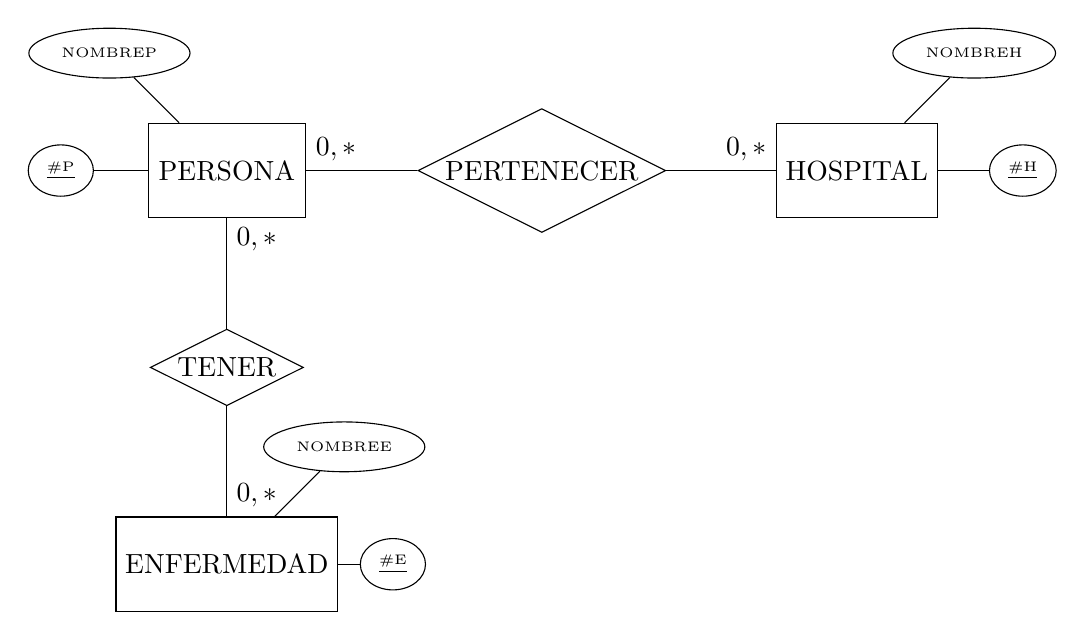
\begin{tikzpicture}[node distance=6em]

        \tikzstyle{every entity} = [minimum width=2cm, minimum height=1.2cm]
        
        
        \node[entity] (estudiante) {PERSONA}
            [sibling distance=3cm]
            child {node[attribute] [above left of=estudiante] {\tiny NOMBREP}}
            child {node[attribute] [left of=estudiante] {\underline{\tiny \#P}}};
      
        \node[entity] (asignatura) at (8,0) {HOSPITAL}
        [sibling distance=3cm]
        child {node[attribute] [right of=asignatura] {\underline{\tiny \#H}}}
        child {node[attribute] [above right of=asignatura] {\tiny NOMBREH}};
        
      
        \node[relationship,aspect=2] (evaluar) at (4,0) {PERTENECER};
        \draw (evaluar.east) -- (asignatura.west) node[above left] {$0,\ast$};
        \draw (evaluar.west) -- (estudiante.east) node[above right] {$0,\ast$};


        \node[entity] (enfermedad) at (0,-5) {ENFERMEDAD}
            [sibling distance=3cm]
            child {node[attribute] [above right of=enfermedad] {\tiny NOMBREE }}
            child {node[attribute] [right of=enfermedad] {\tiny \underline{\#E}}};

        \node[relationship,aspect=2] (tener) at (0,-2.5) {TENER};
        \draw (tener.north) -- (estudiante.south) node[below right] {$0,\ast$};
        \draw (tener.south) -- (enfermedad.north) node[above right] {$0,\ast$};

    \end{tikzpicture}
\end{frame}

\begin{frame}{Definiendo el esquema universal}


    \begin{enumerate}
        \item $U = \{ \textnormal{\#P, NombreP,  \#H, NombreH, \#E, NombreE}\}$
        \item $F = \{$ \\
        \hspace{10mm} $\textnormal{\#P} \to \textnormal{NombreP}$\\
        \hspace{10mm} $\textnormal{\#H} \to \textnormal{NombreH}$\\
        \hspace{10mm} $\textnormal{\#E} \to \textnormal{NombreE}$\\
        \hspace{10mm} $\textnormal{\#P,\#H} \to \textnormal{\#P,\#H}$\\
        \hspace{10mm} $\textnormal{\#P,\#E} \to \textnormal{\#P,\#E}$\\
        $\}$
        \item Definimos el esquema relacional $\textbf{Evaluaciones}(U,F)$ con llave \#P, \#H, \#E
    \end{enumerate}

    \onslide<2>{
        \vspace{5mm}
        \centering
        \large Ya $F$ es un cubrimiento minimal
    }

\end{frame}

\begin{frame}{Obteniendo una descomposici\'on en 3FN}

    \centering
    \begin{columns}[T]
        \begin{column}{0.48\linewidth}
            $R_1(U_1,F_1)$:\\
            \indent $U_1 = \{\textnormal{\#P, NombreP}\}$\\
            \indent $F_1 = \pi_{U_1}(F)$\\[2mm]
            $R_2(U_2,F_2)$:\\
            \indent $U_2 = \{\textnormal{\#H, NombreH}\}$\\
            \indent $F_2 = \pi_{U_2}(F)$\\[2mm]
            $R_3(U_3,F_3)$:\\
            \indent $U_3 = \{\textnormal{\#E, NombreE}\}$\\
            \indent $F_3 = \pi_{U_3}(F)$
        \end{column}
    
    
        \begin{column}{0.48\linewidth}
            $R_4(U_4,F_4)$:\\
            \indent $U_4 = \{\textnormal{\#P, \#H}\}$\\
            \indent $F_4 = \pi_{U_4}(F)$\\[2mm]
            $R_5(U_5,F_5)$:\\
            \indent $U_5 = \{\textnormal{\#P, \#E}\}$\\
            \indent $F_5 = \pi_{U_5}(F)$
        \end{column}
        
    \end{columns}

    \onslide<2>{
        \vspace{8mm}

        \centering
        \Large \it Mira en pizarra c\'omo al unir no se obtiene la original...
    }
\end{frame}

\begin{frame}{Propiedad de Preservaci\'on de Dependencias Funcionales (PPDF)}
    Si para un $R(U,F)$ se tiene la descomposici\'on $\rho = (R_1,R_2,...,R_k)$,
    se dice que $\rho$ cumple la Propiedad de Preservaci\'on de Dependencias Funcionales (PPDF)
    con respecto al conjunto de dependencias funcionales $F$ si:

    $$
        F \equiv \overset{k}{\underset{i=1}{U}} \Pi_{R_i}(F) 
    $$
\end{frame}

\begin{frame}{Recordando}
    \framesubtitle{Algoritmo para obtener una descomposici\'on en 3FN}
    \textbf{Entrada:} Un esquema relacional $R(U,F)$, $F$ es un conjunto irreducible de dependencias funcionales.\\
    \textbf{Salida:} Una descomposici\'on $\rho = (R_1,R_2,...,R_n)$, tal que
    los esquemas relacionales $R_i(U_i,F_i)$ est\'an en 3FN con respecto
    a $\Pi_{R_i}(F)$, $\forall i = 1,...,n$.\\

    \textbf{M\'etodo:}\begin{enumerate}
        \item Crear un esquema por cada dependencia funcional. Preferiblemente, hacer que en el mismo esquema coincidan todas las dependencias funcionales con el mismo miembro izquierdo. Sean estos esquemas $R_1, R_2, ..., R_n$.
        \item Si en $U$ existe alg\'un atributo que no est\'a contenido en ninguna dependencia
        funcional de $F$, este atributo puede formar un esquema relacional por s\'i mismo.
        \item Luego, $\rho = (R_1,R_2,...,R_n)$
    \end{enumerate}
\end{frame}

\begin{frame}{Entonces...}
    \centering
    El algoritmo para obtener una descomposici\'on en 3FN siempre cumple la PPDF
    \vspace{5mm}

    \centering
    ¿Ocurrir\'a lo mismo con la PLJ?
\end{frame}

\begin{frame}{Propiedad del Join sin P\'erdida de Informaci\'on}
    Si para un esquema relacional $R(U,F)$ se tiene la descomposici\'on
    $\rho = (R_1,R_2,...,R_k)$, se dice que dicha descomposici\'on $\rho$ cumple
    con la propiedad de join ($\Join$) sin p\'erdida de informaci\'on con respecto al
    conjunto de dependencias funcionales $F$ si para toda instancia $r$ de $R$ que
    satisfaga a $F$, se cumple que:
    
    $$
        r = \pi_{R_1}(r) \Join \pi_{R_2}(r) \Join ... \Join \pi_{R_k}(r) = \overset{k}{\underset{i=1}{\Join }}R_i(r)
    $$
    
    \vspace{5mm}
    
    \only<2>{
    \begin{center}
        \Large \textcolor{red}{Ya vimos un ejemplo en el que no se cumple :O}
    \end{center}

    }
\end{frame}

% @TODO poner de nuevo lo q es un disenyo correcto 




\begin{frame}{La PLJ es un poco enga\~nosa...}
    \centering
    \Large Requiere que se pueda reconstruir la relaci\'on universal pero...
    \vspace{5mm}

    \centering
    \Large ¿Siempre tiene sentido tener una relaci\'on universal?
\end{frame}

\begin{frame}{Otra forma de comprobar la PLJ}
    \begin{block}{Teorema de Ullman}
        Si $\rho = (R_1,R_2)$ es una descomposici\'on de $R(U,F)$ entonces
        $\rho$ cumple con la PLJ respecto a $F$ si y solo si:
        
        $$
            R_1 \cap R_2 \to R_1 - R_2 \lor R_1 \cap R_2 \to R_2 - R_1
        $$
        
    \end{block}
\end{frame}


\begin{frame}{Un parche para el algoritmo de 3FN que cumple la PPDF}
    \begin{block}{Lema de Ullman}
       Sea $\rho$ una descomposici\'on en 3FN para $R(U,F)$ construida utilizando
       el algoritmo para obtener una descomposici\'on en 3FN que cumple la PPDF, y sea
       $X$ una llave del esquema $R(U,F)$.
       Entonces, $\sigma = \rho \cup {X}$ es una descomposici\'on de $R(U,F)$ con todos sus
       esquemas relacionales en \textcolor{red}{3FN} que cumple la \textcolor{red}{PPDF}, pero que adem\'as cumple con la 
       \textcolor{red}{PLJ}.

    \end{block}

    \onslide<2>{
        \vspace{5mm}

        \centering
        \textcolor{red}{\large Una descomposici\'on obtenida con el algoritmo de 3FN y PPDF siempre puede ser convertida en un dise\~no correcto}
    }
\end{frame}

\begin{frame}
    \frametitle{?`La 3FN siempre elimina las anomal\'ias?}

    \pause

    \begin{align*}
        U &= \{Persona, TipoEstablecimiento, EstablecimientoM\acute{a}sCercano\}  \\
        F &= \{ \\
          & Persona \ TipoEstablecimiento \rightarrow  EstablecimientoM\acute{a}sCercano;\\
          & EstablecimientoM\acute{a}sCercano \rightarrow TipoEstablecimiento \\
          \} &
    \end{align*}

    \pause

    \begin{columns}[c]
        \begin{column}{0.5\textwidth}
    {\Large 
    $R(U, F)$:
    \begin{itemize}[<+->]
        \item[\checkmark] 1FN
        \item[\checkmark] 2FN
        \item[\checkmark] 3FN
    \end{itemize}
    }
        \end{column}
        \begin{column}{0.5\textwidth}
            \centering
            \only<6>{
            \huge \textcolor{red}{?`anomal\'ias?}
            }
        \end{column}
    \end{columns}
\end{frame}

\begin{frame}
    \frametitle{?`Es suficiente con la 3FN?}

    \begin{align*}
        F &= \{ \\
          & Persona \ TipoEstablecimiento \rightarrow  EstablecimientoM\acute{a}sCercano;\\
          & \textcolor<2>{red}{EstablecimientoM\acute{a}sCercano \rightarrow TipoEstablecimiento} \\
          \} &
    \end{align*}

    \begin{table}
        \centering
        \begin{tabular}{|c|c|c|}
            \hline
             \textbf{Persona} &  \textbf{Tipo de Establecimiento} & \textbf{Establecimiento M\'as Cercano} \\\hline
             Claudia & \textcolor<2>{red}{\'Optica} & \textcolor<2>{red}{Almendares}\\\hline
             Claudia & Peluquer\'ia & Luly Sal\'on\\\hline
             Javier & Librer\'ia & Cuba Va\\\hline
             Alejandra & Panader\'ia & La Cubana\\\hline
             Alejandra & Peluquer\'ia & Riudi Peluqueros\\\hline
             Alejandra & \textcolor<2>{red}{\'Optica} & \textcolor<2>{red}{Almendares}\\\hline
        \end{tabular}
    \end{table}

    \vspace{1mm}

    \centering
    \only<2>{
        \huge \textcolor{red}{redundancia}
    }

\end{frame}

\begin{frame}{M\'as all\'a de la 3FN}
    \begin{itemize}
        \item Forma Normal de Boyce-Codd
        \item 4ta Forma Normal
        \item 5ta Forma Normal
    \end{itemize}
\end{frame}
    \begin{frame}
    \centering
    \Huge \textcolor{blue3}{SQL}

\end{frame}

\begin{frame}
	
	\frametitle{Motivación. Estadística en EEUU}
	
	\begin{figure}[h]
		\centering
		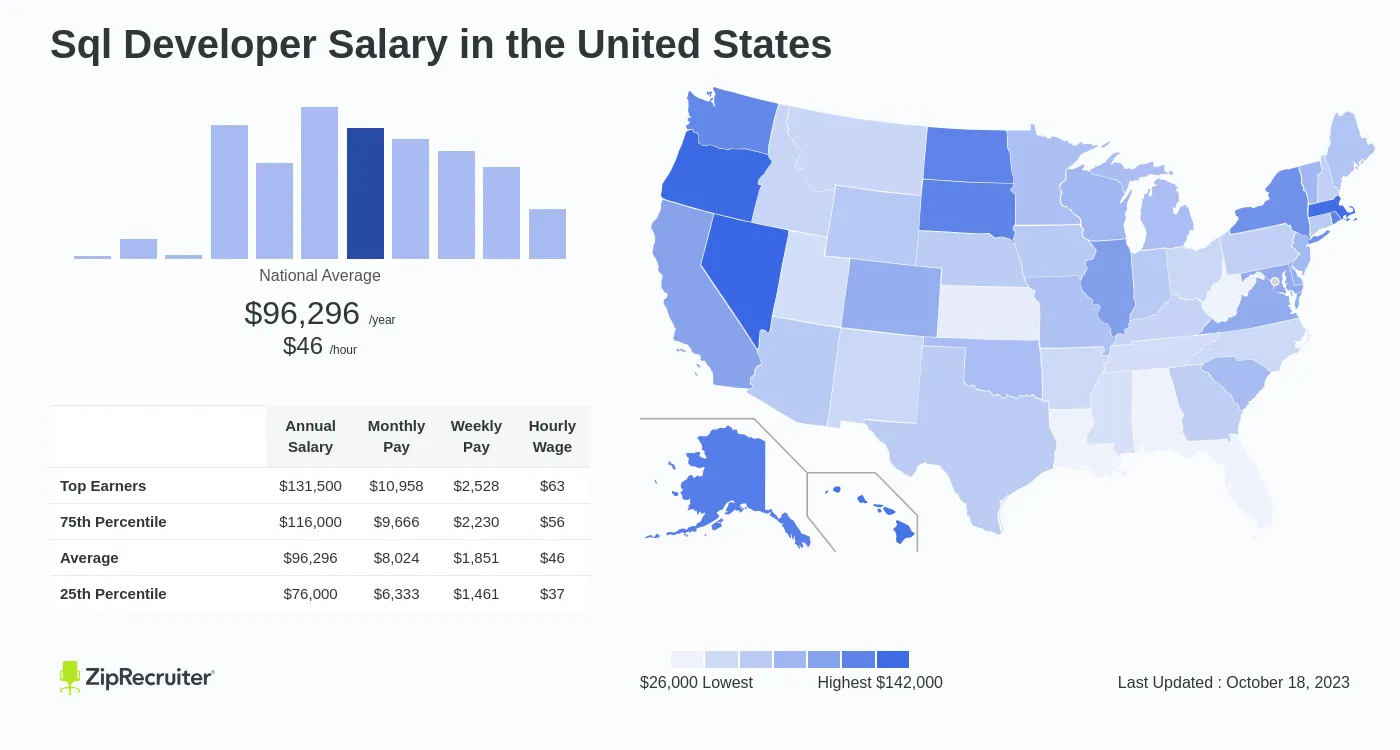
\includegraphics[scale=0.25]{sql-developer-salary.png}
	\end{figure}
	
\end{frame}

%------------------------------------------------

\begin{frame}
	
	\frametitle{Motivación. Estadística en EEUU}
	
	\begin{figure}[h]
		\centering
		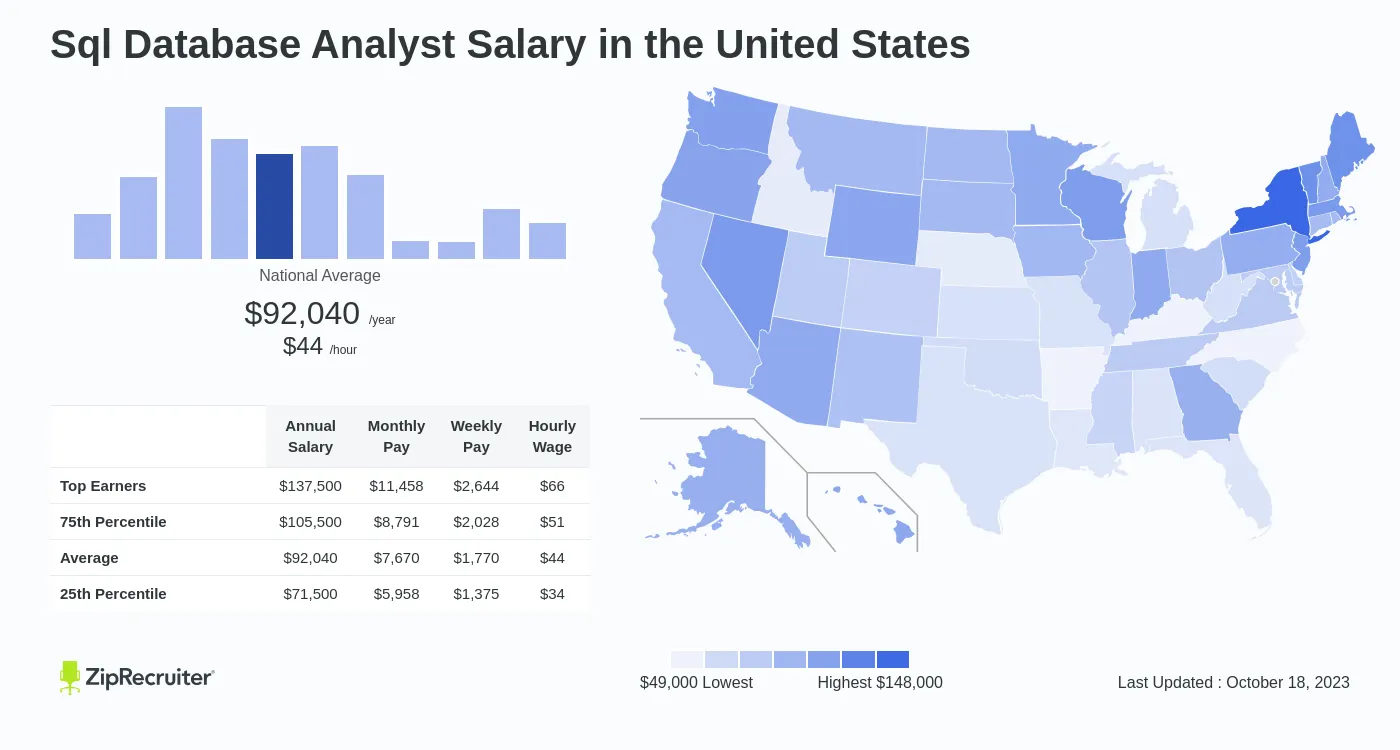
\includegraphics[scale=0.25]{sql-database-analyst-salary.png}
	\end{figure}
	
\end{frame}

%------------------------------------------------

\begin{frame}
	
	\frametitle{Motivación. Estadística en EEUU}
	
	\begin{figure}[h]
		\centering
		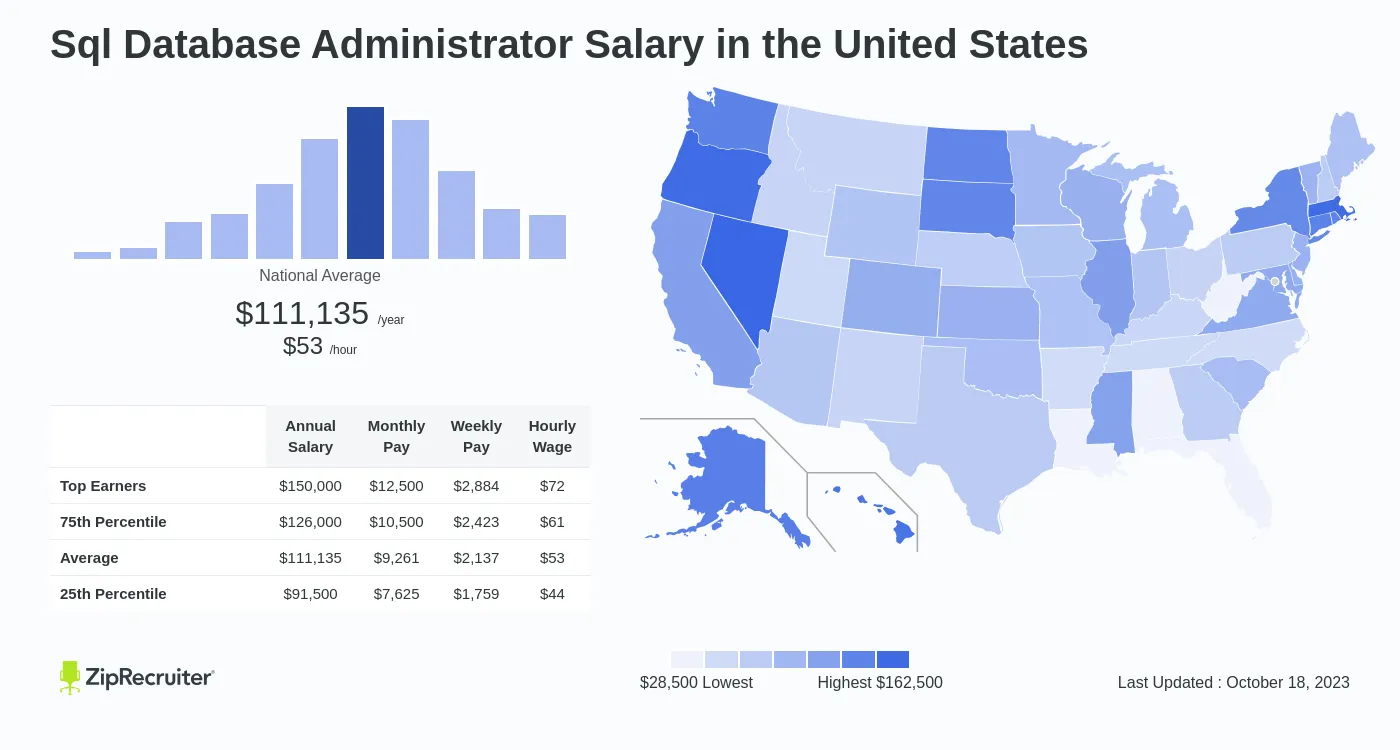
\includegraphics[scale=0.25]{sql-database-administrator-salary.png}
	\end{figure}
	
\end{frame}

%------------------------------------------------

\begin{frame}

	\frametitle{Fundamentos de SQL}
	
	\begin{center}
		\textbf{SQL} 
	
		Structured Query Language
	\end{center}
	
	\pause
	
	\begin{itemize}[<+->]
	
		\item Lenguaje de consulta dise\~nado espec\'ificamente para trabajar con bases de datos relacionales
		\item Lenguaje declarativo
		\item Desarrollado a partir de la década de 1970 por IBM, posterior a la definición del modelo relacional
		\item Desde su creaci\'on, se ha estandarizado a tal punto que es el lenguaje base de muchos otros Sistemas de Gestión de Bases de Datos (MySQL, SQL Server, MS Access, Oracle, Sybase, Informix, Postgres)

	\end{itemize}
	
	\note<5>{@NOTE
		Pudiese decir que es el lenguaje que más se utiliza, puesto que todos los sistemas, independiente de la tecnología que use, si trabaja con base de datos relacionales, es muy probable que use directa o indirectamente SQL.
		
		Es un lenguaje maduro, basado en el álgebra relacional, con poca discrepancias entre sus versiones. Es muy requerido en la vida laboral. 
		
		Si analizamos ciertos aspectos, podemos entender porqué no es un lenguaje de programación. 
		- enfocado en datos, no en operaciones. Sirve para definir, manipular y acceder a los datos almacenados en bases de datos.
		- no puede realizar tareas propias de la programación como bucles, condicionales, declaración de variables, etc.
		- no permite abstraer la lógica de negocio en objetos, clases y métodos como en la programación orientada a objetos.
		- es un estándar implementado por diferentes motores de bases de datos, no un lenguaje de programación como Java, Python, etc.
		- se utiliza en combinación con lenguajes de programación para acceder y gestionar bases de datos desde aplicaciones externas.
	}

\end{frame}

%------------------------------------------------

\begin{frame}

	\frametitle{Componentes de SQL}
	
	
	\begin{itemize}
	
		\item Catálogo de datos

	\end{itemize}
	
	\begin{figure}[h]
		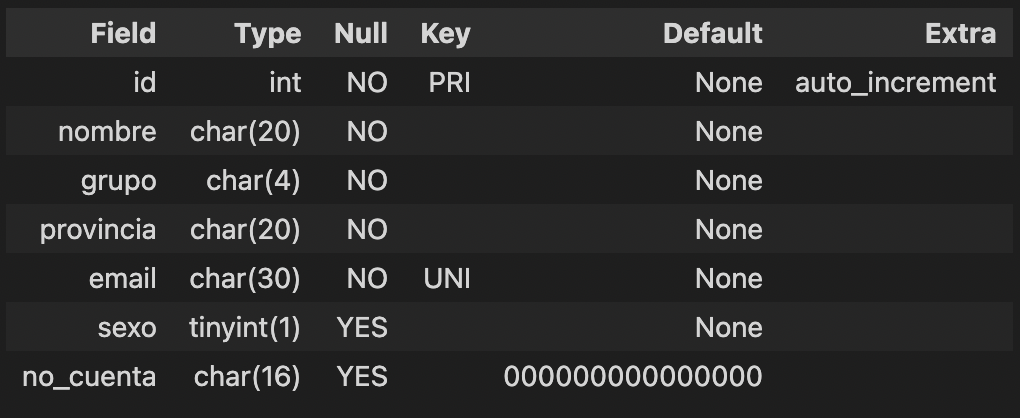
\includegraphics[scale=0.45]{describe.png} Descripción de la tabla
		Datos de la tabla 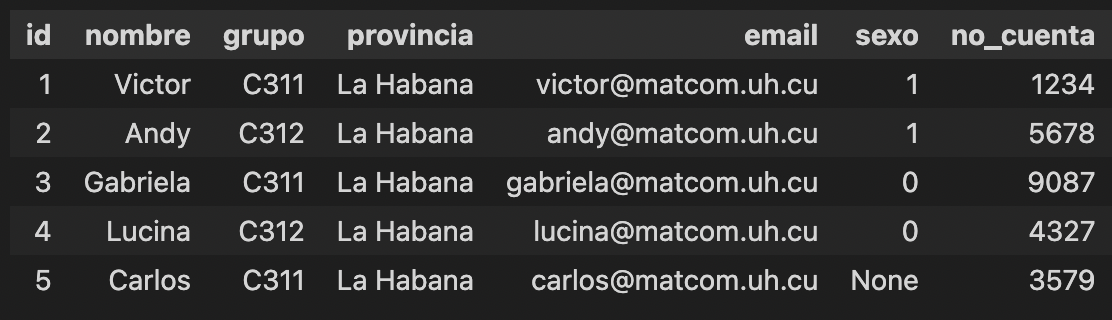
\includegraphics[scale=0.45]{datos.png} 
	\end{figure}

\end{frame}


%------------------------------------------------

\begin{frame}
	
	\frametitle{Componentes de SQL}
	
	
	\begin{itemize}
		
		\item Comandos u órdenes
		\begin{itemize}
			\item<2-> Palabras o frases reservadas: $FROM$, $PRIMARY\ KEY$
			\item<3-> Constantes numéricas y literales.
			\item<4-> Variables: Nombre de tablas y atributos
			\item<5-> Operadores: 

			\only<6->{
			\begin{itemize}
				\item Numéricos: $-$, $+$, $*$
				\item Lógicos: $AND$, $OR$, $NOT$
				\item Relacionales: $<$, $<=$, $>=$, $>$, $=$, $<>$
				\item De cuantificación: $ALL$, $ANY$, $EXIST$
			\end{itemize}
			}
			
		\item<7-> Claúsulas específicas: $BETWEEN$, $IN$, $LIKE$, $DISTINCT$, $IS\ NULL$
		\item<8-> Funciones propias ($SUM$, $IFNULL$) y creadas por el desarrollador
		\item<9-> Restricciones de integridad: $FOREIGN\ KEY$
			
		\end{itemize}
		
	\end{itemize}
	
\end{frame}

%------------------------------------------------

\begin{frame}
	\frametitle{Tipos de comandos}
	
	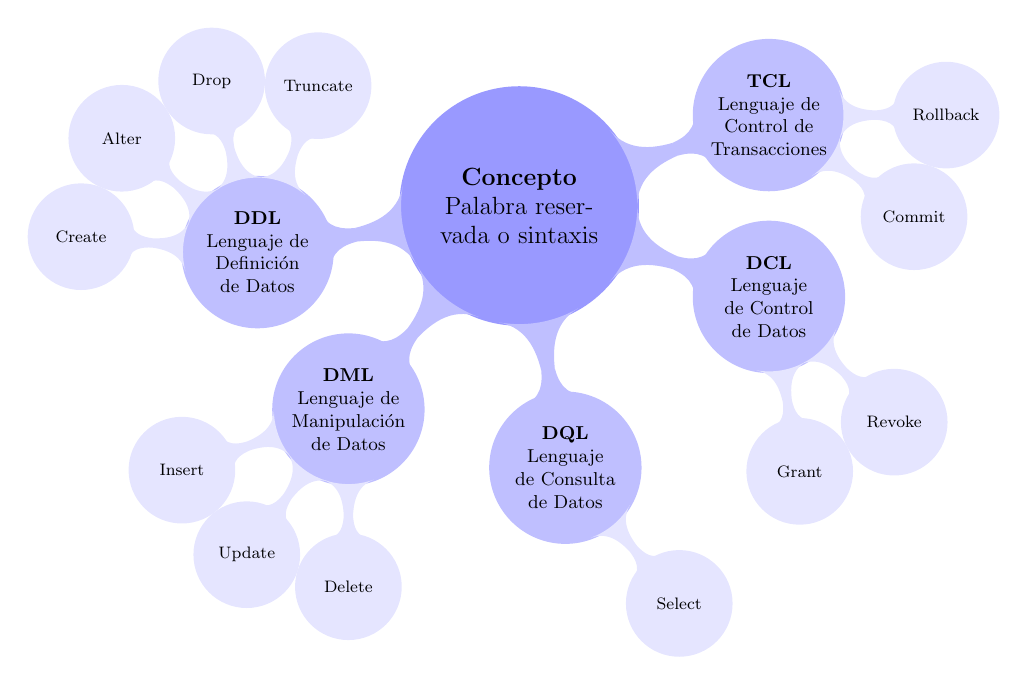
\begin{tikzpicture}[
		scale=0.75,
		transform shape,
        		mindmap,
        		concept color = blue!40,
        		every node/.style = {concept},
        		grow cyclic,
        		level 1/.append style = {
            		concept color = blue!25,
           		level distance = 4.5cm,
            		sibling angle = 120
        		},
       		level 2/.append style = {
            		concept color = blue!10,
            		level distance = 3cm,
            		sibling angle = 45
        		}
    	]
    	\node [concept] at (current page.center) {\textbf{Concepto} \\ Palabra reservada o sintaxis}
    	child[grow=190]{
        		node {\textbf{DDL} \\ Lenguaje de Definici\'on de Datos}
		child[grow=175]{node {Create}}
		child[grow=140]{node {Alter}}
		child[grow=105]{node {Drop}}
		child[grow=70]{node {Truncate}}
         }
         child[grow=230]{
         	node {\textbf{DML} \\ Lenguaje de Manipulaci\'on de Datos}
         	child[grow=200]{node {Insert}}
         	child[grow=235]{node {Update}}
         	child[grow=270]{node {Delete}}
         }
         child[grow=280]{
        		node {\textbf{DQL} \\ Lenguaje de Consulta de Datos}
		child[grow=310]{node {Select}}
         }
         child[grow=340]{
        		node {\textbf{DCL} \\ Lenguaje de Control de Datos}
		child[grow=315]{node {Revoke}}
		child[grow=280]{node {Grant}}
         }
         child[grow=20]{
        		node {\textbf{TCL} \\ Lenguaje de Control de \\ Transacciones}
		child[grow=0]{node {Rollback}}
		child[grow=325]{node {Commit}}
         }
        ;
	\end{tikzpicture}
	
	\note{@NOTE
		DDL se refiere a comandos SQL que diseñan la estructura de la base de datos.
		DQL consiste en instrucciones para recuperar datos almacenados en bases de datos relacionales.
		DML escriben información nueva o modifican los registros existentes en una base de datos relacional.
		DCL  administra o autoriza el acceso a la base de datos.
		TCL hace cambios en la base de datos de manera automática. 
	}

\end{frame}

%------------------------------------------------

\begin{frame}

	\frametitle{Jugando con SQL}
	
	Auxiliarse del fichero \alert{Conferencia\_6.ipynb} % @TODO cambiar nombre


\end{frame}

%------------------------------------------------

\begin{frame}

	\frametitle{Tipos de datos}

	\begin{columns}[c] 
		\begin{column}{0.45\textwidth} % Left column width
			\begin{itemize}
	
				\item<2-> Numéricos
				\only<2->{
					\begin{itemize}
					\item INT
					\item BIT o BOOLEAN
					\item MONEY
					\item FLOAT
				\end{itemize}
				}
			
			\item<3-> Cadenas de caracteres
				\only<3->{
				\begin{itemize}
					\item CHAR o NCHAR
					\item VARCHAR o NVARCHAR
			\end{itemize}

				}
			
			\item<4-> Cadenas binarias
			\only<4->{
				\begin{itemize}
					\item BINARY
				\end{itemize}

			}
			
		\end{itemize}
		\end{column}
		
		\begin{column}{0.5\textwidth} % Right column width
		\begin{itemize}
		
			\item<5-> Fecha y hora
			\only<5->{
			\begin{itemize}
				\item DATE				
				\item TIME
				\item DATETIME
			\end{itemize}
			}
			
			\item<6-> Otros
			\only<6->{
			\begin{itemize}
				\item XML				
				\item GEOGRAFÍA ESPACIAL
			\end{itemize}

			}
			
		\end{itemize}			
		\end{column}
		
	\end{columns}

	\vspace{5mm}

	\centering
	\only<7->{
	\Large \textcolor{red}{Consultar manual de SQL}
	}

\end{frame}

%------------------------------------------------

\begin{frame}

	\frametitle{Restricciones de integridad}
	
	\note{@NOTE
		- Reglas y restricciones predefinidas, muchas veces a raíz de las reglas del negocio. 
		- Se aplican por columna.
		- La operación de inserción se efectúa, solo si se cumple todas las restricciones definidas.
		- 
	}
	
	\begin{itemize}
		\item<2-> PRIMARY KEY
		\item<3-> FOREIGN KEY	
		\only<3->{
			\begin{itemize}
				\item Activadores: ON UPDATE, ON DELETE
				\item Modificadores: CASCADE, RESTRICT, SET NULL, SET DEFAULT, NO ACTION
			\end{itemize}
		}
		
		\item<4-> NOT NULL 
		\item<5-> UNIQUE
		\item<6-> CHECK \textit{condici\'on}
		\item<7-> DEFAULT	\textit{valor}
	
	\end{itemize}
	
	

\end{frame}

%------------------------------------------------

\begin{frame}
	
	\frametitle{Dudas, comentarios, sugerencias}
	
	\begin{figure}[h]
		
\includegraphics[scale=0.4]{duda.jpg}
	\end{figure}
	
	

\end{frame}
    \maketitle
\end{document}
